\documentclass{article}
\usepackage[T1]{fontenc}
\usepackage{lmodern}
\usepackage{graphicx}
\usepackage{amsmath,amssymb}
\usepackage[a4paper,margin=2cm]{geometry}
\usepackage[absolute,overlay]{textpos}
\setlength{\TPHorizModule}{1mm}
\setlength{\TPVertModule}{1mm}
\usepackage[indonesian]{babel}
\usepackage{hyperref}
\setlength{\emergencystretch}{2em}
% unit: Halaman 46

\begin{document}

% === Halaman 46 (llm) ===

Misalkan \underline{semua} bit LSB pada citra berwarna dibalikkan dari semula 0 menjadi 1; dari semula 1 menjadi 0

\vspace{10mm}

\begin{center}
\begin{tabular}{cc}
Sebelum & Sesudah
\end{tabular}
\end{center}

\begin{center}
\textcolor{red}{Adakah terlihat perbedaaannya?}
\end{center}

% deskripsi: Dua buah gambar perbandingan citra berwarna kapal layar, satu sebelum manipulasi bit LSB dan satu setelah manipulasi bit LSB, yang terlihat hampir identik.
% bbox normalisasi: [0.1500, 0.2400, 0.8500, 0.8200]
\begin{textblock*}{147.00mm}(31.50mm,71.28mm)
\noindent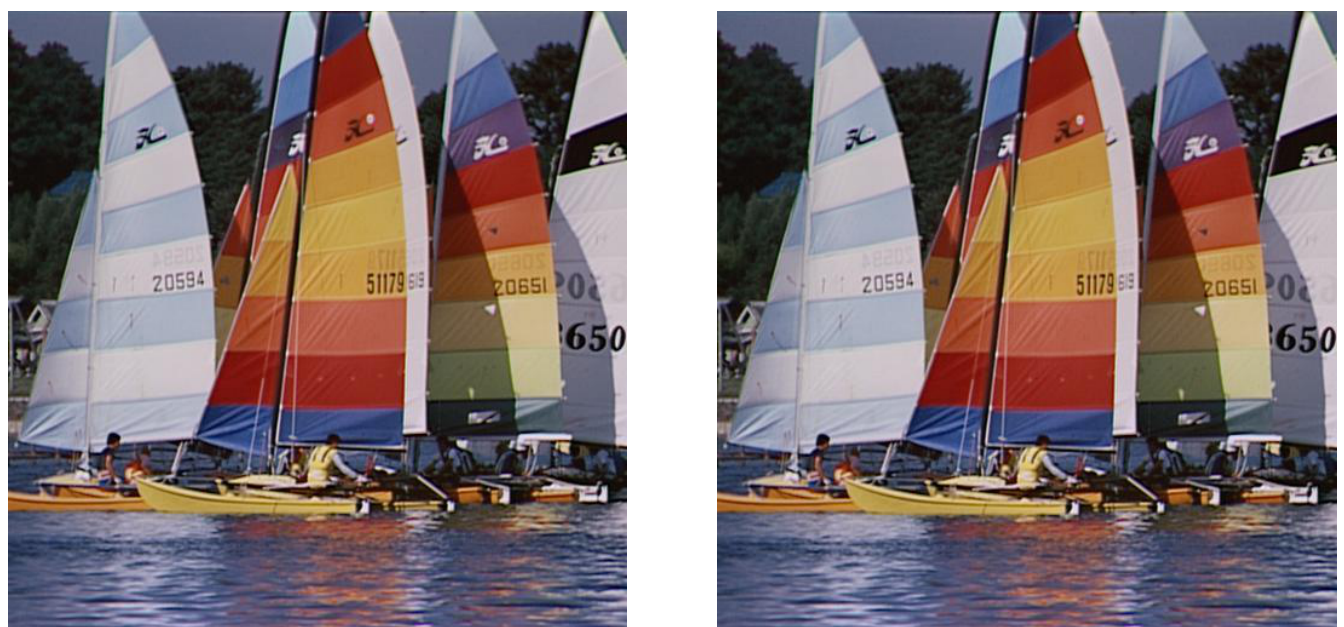
\includegraphics[width=147.00mm,height=172.26mm]{../../images/llm/page_046_img_01.png}%
\end{textblock*}

\end{document}
